%%================================================
%% Filename: chap03.tex
%% Encoding: UTF-8
%% Author: 苏峻锋
%% Created: 2024-02-28
%% Last modified: 2024-02-28
%%================================================
\chapter{网站访问量时间序列预测研究}

Nginx 作为一款高性能的HTTP和反向代理服务器,其本身和时间序列不是直接相关。
但是,在监控Nginx性能的过程中,会涉及到时间序列数据。比如,Nginx的访问日志和错误日志都会记录下请求的时间信息,
这些日志数据就构成了时间序列数据。可以通过分析这些时间序列数据来理解Nginx的流量模式、
性能趋势以及潜在的问题。而且,对于时间序列的处理和分析还可以应用在Nginx及其它服务的自动化监控和告警系统中。
这样的系统可以帮助管理者更有效地了解服务状态,并在出现问题时迅速作出反应。

\section{时间序列预测基本方法}

时间序列是一组按照时间顺序排列的数据点。这种数据点是通常按照固定的时间间隔收集,
比如每天,每周,每月,每年的观测值。间序列数据用在许多领域,包括经济学、气象学、社会学、工程和自然科学等。例如,股票市场价格、气温记录或公司收入都可以被视作时间序列数据。通过对时间序列数据的分析,可以洞察到数据背后的趋势、季节性变化、循环等特征,也可以用来做出未来的预测。
在 Nginx 网络访问量的时间序列数据点则可以将每一天某个网页的访问量记录下来,按照日期的对应关系,每一个 datetime 对应一个 record。

时间序列预测方法有很多,简单的方法不多提,主要研究了指数平滑法、趋势延伸法、自回归滑动平均模型(ARMA)、差分整合移动平均自回归模型(ARIMA)。

(1)指数平滑法是一种预测技术,它根据历史数据的时间序列加权和进行优化改进。此方法按照平滑次数进行分类,包括单一指数平滑、双重指数平滑以及三重指数平滑等多种形式。尽管指数平滑法的核心思想与移动平均法相似,即对时间序列中的历史数据赋予不同的权重,但两者在权重分配上有明显区别。指数平滑法对近期数据赋予更高的权重,而随着时间的推移,对数据的权重递减,以更好地反映近期趋势的影响。

至于趋势延伸法,它通过将时间序列中的历史数据在坐标图上标记出来,随后绘制一条能最佳拟合历史数据变化的线性或非线性趋势线。通过对这条趋势线进行向前延伸,我们可以基于已有的数据模式进行未来数据点的预测,进而提供一种直观的趋势展望。

(2)自回归滑动平均模型\cite{贾钟研2020基于时间序列的网络流量分析与预测}(ARMA)
结合了自回归模型(AR)和滑动平均模型(MA),ARMA模型能有效地捕捉时间序列数据的自相关结构。
AR(p)模型,它预测当前值作为前p个观测值(lags)的线性组合,模型中的p代表模型的阶数,
即延迟的观测值的数量。AR部分的如下所示
\begin{equation}
  X_t = \phi_1X_{t-1} + \phi_2X_{t - 2} + \cdots + \phi_pX_{t-p} + \epsilon_t
\end{equation}
其中,$X-t$ 是时间序列在时刻 t 的值,$\phi_1, \phi_2,\ldots,\phi_p$是模型参数,$\epsilon_t$是白噪声误差项。
MA(q)模型,即移动平均模型,它使用当前和过去的预测误差(即观测值与模型预测值之间的差)来预测当前值。模型中的q代表误差项的阶数。
\begin{equation}
  X_t = \epsilon_t + \theta_1\epsilon_{t-1} + \theta_2\epsilon_{t-2} + \cdots + \theta_q\epsilon_{t-1}
\end{equation}
其中,$\epsilon_t$ 是模型的白噪声误差项,$\theta_1, \theta_2, \ldots, \theta_q$是模型参数。把AR部分和MA部分结合起来就得到了 ARMA 模型。
\begin{equation}
  X_t = \phi_1X_{t-1} + \cdots  + \phi_pX_{t-p} + \epsilon_t + \theta_1\epsilon_{t-1} + \cdots + \theta_q\epsilon_{t-q}
\end{equation}

ARMA模型的参数通常通过极大似然估计(Maximum Likelihood Estimation, MLE)或者最小二乘法来确定。在使用ARMA模型之前,往往需要确定模型的p和q值,这通常通过模型的自相关函数(ACF)和偏自相关函数(PACF)来辅助确定。此外,模型需要时间序列数据是平稳的,如果数据不平稳,往往需要通过差分等手段将其转化为平稳时间序列。

网络访问量的时间序列在一定时间内是比较平缓的,比如在每天的凌晨至第二天上午7点,七点到下午 5 点。这个时间点以外的访问量就比较复杂。遇见节日天气,访问量的预测就愈发困难。ARMA模型适合处理和预测短期的平稳时间序列数据,而在处理非平稳时间序列时,经常会使用ARMA模型的扩展版-ARIMA模型。

(3)自回归差分移动平均模型(ARIMA)。

ARIMA模型是在ARMA模型的基础上增加了差分的操作,以处理非平稳时间序列数据。ARIMA模型的一般形式为ARIMA(p, d, q)。其中,p是自回归项的阶数,d是差分次数,q是移动平均项的阶数。ARIMA模型的一般形式为
\begin{equation}
  (1 - \phi_1B - \cdots - \phi_pB^p)(1 - B)^dX_t = (1 + \theta_1B + \cdots + \theta_qB^q)\epsilon_t
\end{equation}

其中,B是差分操作符,$\phi_1, \phi_2, \ldots, \phi_p$是自回归项的系数,$\theta_1, \theta_2, \ldots, \theta_q$是移动平均项的系数,$\epsilon_t$是白噪声误差项。ARIMA模型的参数通常通过极大似然估计(Maximum Likelihood Estimation, MLE)或者最小二乘法来确定。在使用ARIMA模型之前,往往需要确定模型的p、d和q值,这通常通过模型的自相关函数(ACF)和偏自相关函数(PACF)来辅助确定。ARIMA模型的优点是能够处理非平稳时间序列数据,但是它的缺点是需要对模型的参数进行较为复杂的确定。

\section{访问量的时间序列预测算法}

对于访问量的预测能够有效的对服务器集群的负载能力加以调节,避免访问量过大导致的服务器集群某一节点的负载过高,使得任务处理能力下降,从而达到增强负载均衡的作用。

由于某些限制,没有使用最近几年的网页流量数据作为原始数据。
因此,在本次预测模型测试中,所采用的数据集来源于Kaggle比赛“Web Traffic Time Series Forecasting”提供的网络访问量数据集。
该数据集包含了若干维基条目的日访问量,总计约145,000篇维基百科页面。
类型为train\_.csv的文件包含了流量数据,其中,每一行对应一篇特定的文章,而每一列对应一个特定的日期。
train\_1.csv记录了从2015年7月至2016年12月,共550天内的日访问状况;而train\_2.csv记录了从2015年7月至2017年9月,共803天的日访问情况。
类型为key\_.csv的文件,则提供了用于预测的页面名称与简化ID之间的映射。

训练数据集包含大约145,000个时间序列,每个时间序列表示不同维基百科文章从2015年7月1日至2016年12月31日的每日浏览次数。
每个时间序列都标明了文章标题和流量类别(包括全部、移动端、桌面端和爬虫)。
这项研究结合了额外的元数据和其他公开获取的数据集来进行预测。然而,该数据集并没有区分零流量值与缺失值,缺失值可能代表无流量,或当日数据缺失。
本研究案例选择了“泰勒·斯威夫特”条目页面的访问数据进行分析,如下图\ref{Taylor_swift}所示。

\begin{figure}[htb]
  \centering
  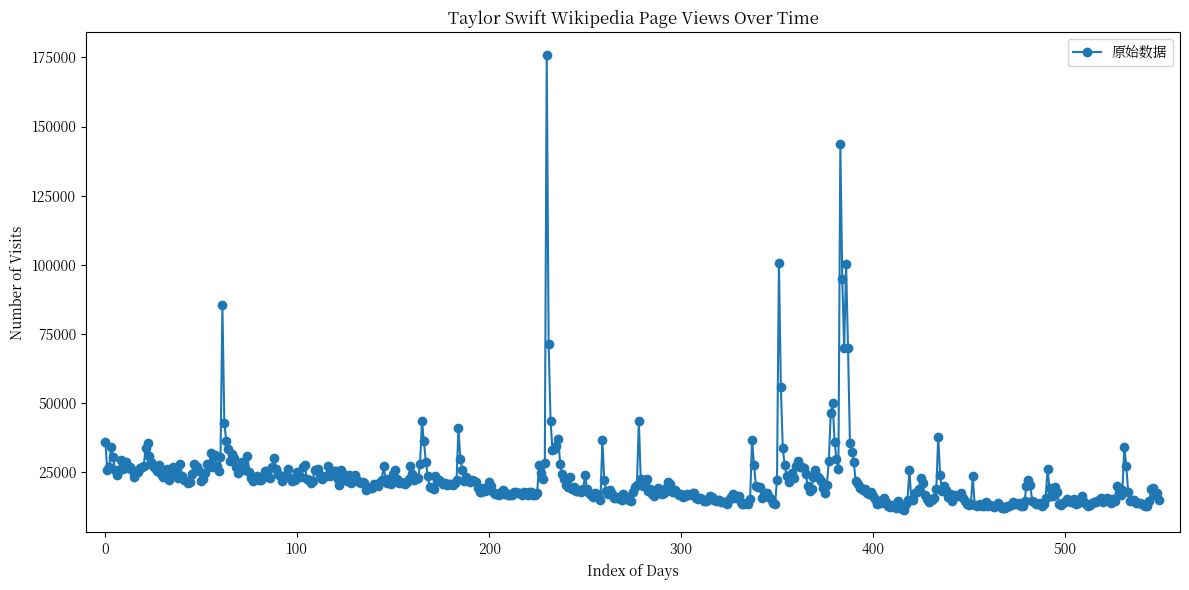
\includegraphics[width=\textwidth]{figures/taylor_source.png}
  \caption{泰勒·斯威夫特日访问量变化}
  \label{Taylor_swift}
\end{figure}

为了能够知道模型的准确地,使用了重要指标 SMAPE(对称平均绝对百分比误差)一种常用于预测精度评估的指标,可以比较不同规模时间序列的误差。计算公式如下。

\begin{equation}
  SMAPE={\frac{100}{n}}\sum_{t=1}^{n}{\frac{|F_{t}-A_{t}|}{(|A_{t}|+|F_{t}|)/2}}
\end{equation}

其中这个公式的 $n$ 是观察总数,$F_t$ 是时间 t 的预测值,$A_t$ 是时间 t 的实际值。
SMAPE的值范围是0\%到200\%,较低的SMAPE值表示较高的预测精度。与其他评估指标相比,它同时考虑了预测值和实际值的误差,避免了过分强调其中一个
SMAPE通过相对误差进行测量,使其不依赖于数据的规模,因此适合比较不同规模的时间序列。

然而,SMAPE也存在一定的局限性,当时间序列的值接近零时,
SMAPE可以变得非常有问题。这是因为当实际值 ( A\_t ) 或预测值 ( F\_t ) 接近于零时,SMAPE的分母会变得很小,即使是很小的绝对误差也会导致很大的百分比误差。下面图3.2是关于 SAMPE 指标的极端测试图。

\begin{figure}
  \centering
  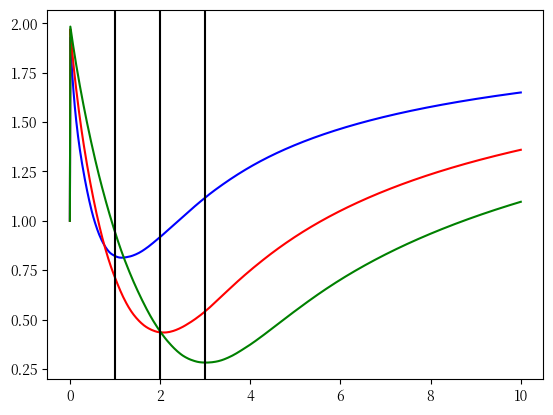
\includegraphics[width=0.8\textwidth]{figures/sampe_external.png}
  \caption{SAMPE 指标极端测试}
  \label{sampe-property}
\end{figure}

在图片\ref{sampe-property}中,垂直的线代表了真实值$1 , 2, 3$ 通过不同真实值的表现体现了 SAMPE 的动态分数。当实际值和预测值的差接近于零是,SMAPE 的分数会接近于无穷,所以要避免这个问题。

\subsection{ARIMA 算法访问量预测}

ARIME 模型也被称为 Box-Jenkins 模型,可能包含自回归项(AR)、移动平均(MA)、
差分运算(I)。

自回归即当前时刻的观察值是之前多个时刻观察值的线性组合加上一个随机误差项。
基本上,自回归的核心思想是,过去的值对未来的值有一定的预测能力,隐含地假设未来将与过去相似。
因为这个核心思想,所以必然的会有一定程度上的缺点。

移动平均(MA)是一种统计手段,用于分析时间序列数据。通过创建一系列平均数来平滑短期波动并突出显示长期趋势或周期。简单的举一个移动平均磨的模型,计算公式为 $SMA = \frac{P_1 + P_2 + \cdots + P_n}{n}$,其中P 是不同时间下的价格或者观察的序列,
而 n 是时间周期的长度即周期内一共有多少观察的时间数目

差分运算(I)在时间序列分析中,是将非平稳时间序列数据转换为平稳数据的方法之一。
若一个时间序列是平稳的,即其统计特性(如均值、方差)不会随时间发生变化。
许多统计模型和预测方法都以平稳性为其重要假设条件。针对非平稳时间序列,可以通过差分运算将其转换成平稳序列。
差分运算主要是计算时间序列中相邻观测值之间的差值。

例如,一阶差分可以用公式 $\Delta Y_t = Y_t - Y_{t - 1}$ 来表示,这是基本且易于理解的运算。如果时间序列在一阶差分后仍不平稳,那么可进一步尝试更高阶的差分操作,如二阶差分,其计算公式为:
\begin{equation}
  \Delta^2 Y_t = (Y_t - Y_{t - 1}) - (Y_{t - 1} - Y_{t - 2})
\end{equation}

一般来说,一阶或二阶差分足以处理大多数的非平稳序列。差分运算是构建ARIMA(自回归积分滑动平均)模型的关键步骤之一

对于 ARIMA 模型来说,可以通过上面三个关键含义来理解这个模型。自回归是指显示变化变量的模型,该变量根据自身的滞后值或者先验值进行回归;差分,表示
原始观测值与先前值的差异,用来使时间序列变得平稳;移动平均结合了观测值与应用于滞后的观测值的移动平均模型之间的残差之间的依赖性

(1)数据的预处理

由于 Kaggle 比赛中使用的数据命名的混乱,比如存在 52\_Hz\_I\_Love\_You\_zh.wikipedia.org\_all-access\_spider 
复杂的命名需要进行重新命名和分类,同时需要填充不存在的数值为 NaN
同时由于 ARIMA 模型对数据进行分析和预测要求序列是有一个零均值平稳随机过程产生,因此需要需要判断数据的平稳性\cite{赵鹏2020基于},通过使用 ADF 检验序列中是否存在单位根,如果存在则为非平稳时间序列。
ADF检验的核心是基于一个时间序列模型来测试序列中的单位根。具体来说,ADF检验通常使用以下的回归模型来进行单位根的测试。
\begin{equation}
    \Delta y_t = \alpha + \beta t + \gamma y_{t-1} + \delta_1 \Delta y_{t-1} + \cdots + \delta_p \Delta y_{t-p} + \epsilon_t
\end{equation}
在这个公式中,$y_t$ 是时间序列数据,$\Delta$ 是一阶差分运算符,$\Delta y_t = y_t - y_{t-1}$,$t$ 是趋势项,$\alpha$是常数项,$\beta$ 是时间趋势项的系数,$\gamma$ 是滞后一阶的系数,ADF检验的关键在于检验这个系数;如果$\gamma = 0$,则存在单位根,$\delta_1, \delta_2, \cdots, \delta_p$ 是差分项的系数,$\epsilon_t$ 是随机误差项,$p$ 是滞后阶数,它可以根据各种信息准则(如AIC或BIC)来确定。下表给出了泰勒·斯威夫特词条进行ADF检验的结果。

\noindent\begin{longtblr}[
  caption = {泰勒·斯威夫特的 ADF 检验},
]{
  width = \linewidth,
  colspec = {Q[312]Q[279]Q[410]},
  cell{1}{1} = {c=2}{0.591\linewidth,c},
  cell{2}{1} = {r=3}{},
  cell{5}{1} = {c=2}{0.591\linewidth,c},
  cell{6}{1} = {c=2}{0.591\linewidth,c},
  hline{1,7} = {-}{0.08em},
  hline{2} = {-}{},
}
参数    &            & 值             \\
测试临界值 & level 1\%  & -3.442361e+00 \\
      & level 5\%  & -2.866838e+00 \\
      & level 10\% & -2.569592e+00 \\
t统计量  &            & -7.674316e+00 \\
P 值   &            & 1.563457e-11  
\end{longtblr}

ADF 的检验结果可知,
ADF 值即 t 统计量远远小于 level 1\%、level 5\%、level 10\%的三个显著性水平条件下的临界值,故该原始序列为平稳时间序列,非常适合 ARIMA 模型来进行预测。

(2)参数标定

根据 ADF 的检验结果得知,该时间序列是一个平稳的时间序列,已经不需要进行差分,所以参数 d 即原始观测值差异的次数;也称为差异度为 0。
而 q 和 p 的数值则需要通过自相关及偏自相关函数来进行判断。

在时间序列分析中,p和 q 是ARIMA模型(自回归差分移动平均模型)的关键参数\cite{TJJC201923008},
其中p代表自回归(AR)项的阶数,它是过去值的数量, q代表移动平均(MA)项的阶数,它是预测误差的数量。
为了得到合适的 p 和 q 值,自相关函数(ACF)为移动平均组件 q 提供界限。ACF 图显示了时序和它自己滞后版本之间的相关性。
偏自相关函数(PACF):为自回归组件 p 提供界限。PACF 图仅显示不被更早滞后项解释的当前滞后项的相关性。自相关和偏自相关函数系数和滞后值关系如下:

\begin{figure}[htb]
  \centering
  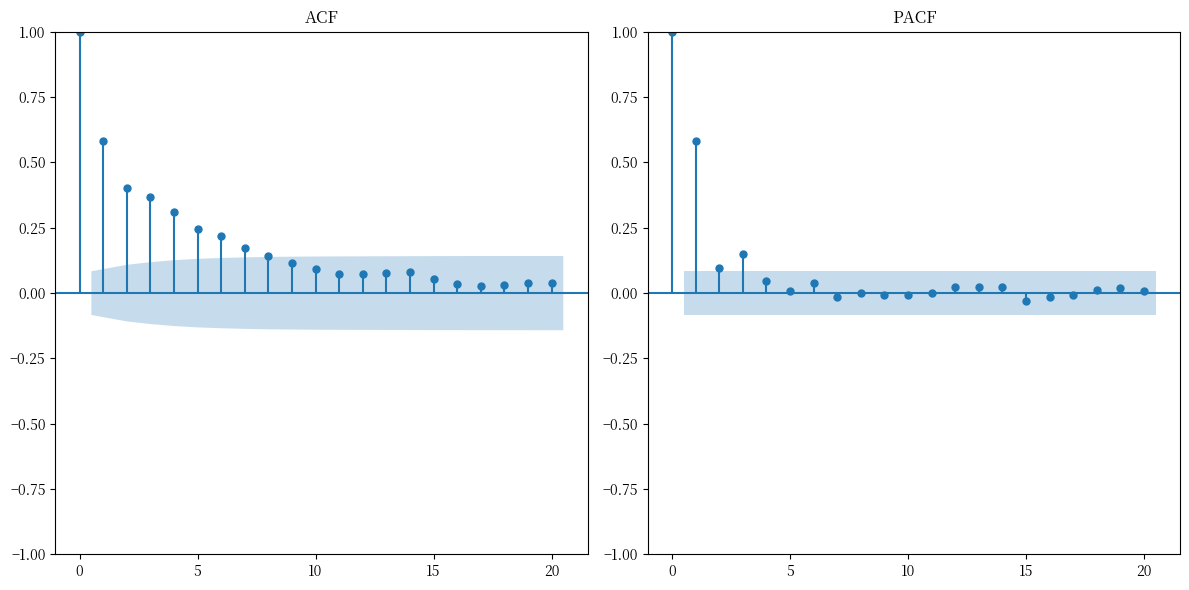
\includegraphics[width=\textwidth]{figures/acf_pacf.png}
  \caption{ACF 与 PACF 相关系数和滞后值的联系}
\end{figure}

如图3.2 所示,x 值即滞后值,y 值即相关系数,蓝色的区域是显著性水平分界线,如果在蓝色之内则是非显著的,
因为我们必须要对数据具有显著性的要求,毕竟如果没有显著性的差异,也就很难有什么变化或者预测了。ACF 图和 PACF 表示的是一个 AR 过程和 MA 过程一个相关性不断减小的过程。
当PACF图在滞后数p之后截尾,即相关性突然下降到不显著水平,则可以用来辨识AR模型的阶数p即为2; 当ACF图在滞后数q之后截尾即相关性突然下降到不显著水平,则可以用来辨识MA模型的阶数q 即为 1。利用 Python 对该模型的个参数进行估计,得到参数估计结果见表3.6。

\noindent\begin{longtblr}[
  caption = {ARIMA 模型拟合结果},
]{
  width = \linewidth,
  colspec = {Q[292]Q[173]Q[237]Q[173]},
  hline{1,6} = {-}{0.08em},
  hline{2} = {-}{},
}
模型     & 系数    & t 统计量   & P 值   \\
AR(1)  & 0.169 & 6.796   & 0.000 \\
AR(2)  & 0.107 & -2.310  & 0.021 \\
MA(1)  & 0.163 & -4.059  & 0.000 \\
SMA(2) & 3.086 & 3.4e+07 & 0.000 
\end{longtblr}

其中 $p$ 值是一个统计假设检验的概念,帮助决定观察到的数据是否显著性的与假设矛盾,进而否定这个假设。如果 $p$ 值很小,小于 0.05 那么就说结果具有统计学上的显著性,这表示出现极端数据的概率很低,反之则没有统计学上的相关性,很难找到统计学上的意义。
可以看出 ARIMA(2,0,1)在 1\%的显著水平下,AR(1)、AR(2)、MA(1)、SMA(2)的相关系数显著不为 0,回归系数的 $p$ 值均小于 0.05,所以对于 泰勒斯威夫特这个词条,通过了显著性检验。

已经确定了 $p$, $d$, $q$, 的值,则可以直接对泰勒·斯威夫特的时间进行预测,图3.4 是泰勒·斯威夫特的ARIMA预测值与实际值的对比。

\begin{figure}[htb]
  \centering
  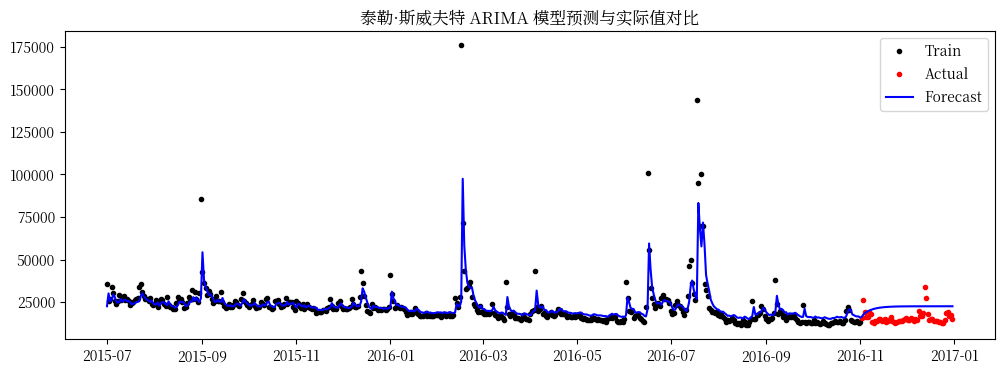
\includegraphics[width=\textwidth]{figures/taylor_arima.png}
  \caption{泰勒·斯威夫特词条 ARIMA 模型预测结果}
\end{figure}

可以看到蓝色的线条基本覆盖掉原始的训练实际值,但是在使用拟合的模型来进行预测的时候,可以看到蓝色的线条并不能很好的覆盖掉真实的实际值即模型仍旧没有很好的预测到真实的实际情况,需要进一步的分析研究。

在某些场景下,ARIMA模型通常被认为是适用于短期预测的,自回归部分依赖于时间序列的先前值,而移动平均则依赖于预测误差的先前值。因此,模型特别关注数据中的局部波动,而这些往往在短期内更加稳定。
但是在长期预测场景下,可能存在许多不可预测的外部因素和趋势变化,这些因素很难被ARIMA模型所捕捉。为了解决上述问题,让时间序列更好的得到预测,笔者使用了 Facebook 的 prophet 模型对词条进行预测。

\subsection{Facebook prophet 算法访问量预测}

Facebook的Prophet模型是一个开源的时间序列预测工具,由Facebook的Core Data Science团队开发\cite{taylor2018forecasting}。
Prophet的设计目标是让时间序列的预测工作变得更加简单,并且它对于具有强季节性效应的历史数据尤其适用。
它在处理缺失数据和异常值方面具有鲁棒性,并且能容忍时间序列中的一些非常规变化,因此对实际应用场景非常友好。此外,Prophet还支持添加重要的节假日效应。

Prophet模型在使用上很灵活,使得用户可以根据自己的需求和熟悉的环境来选择合适的工具进行预测。
Prophet背后的模型基础是一个可加性模型,其中趋势、季节性和节假日效应可以分解非常清晰地展示出来,这使得模型的结果很容易解释。

在时间序列分析中,一个常用的方法是时间序列分解,该方法将时间序列 $y_{t}$,分解为几个组成部分,它们是季节性项 $S_{t}$、
趋势项 $T_{t}$ 和残差项 $R_{t}$;在实际应用中,除了季节性、趋势性和残差这三个因素外,节假日效应也是不能忽视的因素。
因此,在Prophet算法中,将这四个成分纳入考虑,即 $y(t) = g(t) + s(t) + h(t) + \epsilon_{t}$,这样做提供了更全面的时间序列预测。

其中,$g(t)$ 代表时间序列的长期趋势,反映了时间序列在非周期性变化下的总体走向;$s(t)$ 代表时间序列的周期性变动,通常以周或年为周期;$h(t)$ 则体现了节假日在当天是否存在以及节假日效应的强弱;
$\epsilon_{t}$ 为误差项,刻画了模型未能解释的随机波动。Prophet算法通过拟合趋势项、季节项、节假日项,将它们叠加得到时间序列的预测值,从而实现对未来的预估。

(1)趋势项 $g(t)$

在 Prophet 算法里面,趋势项有两个重要的函数,一个是基于逻辑回归函数(logistic function)的,
另一个是基于分段线性函数(piecewise linear function)的。

在逻辑回归函数中,一般形式是 $\sigma(x) = 1/(1+e^{-x})$ ,它的导数是 $\sigma'(x) = \sigma(x) \cdot(1-\sigma(x))$,而且$\lim_{x\rightarrow +\infty} \sigma(x) = 1, \lim_{x\rightarrow -\infty} \sigma(x) = 0$。
如果增加一些参数的话,那么逻辑回归就可以改写成如下方程\cite{李威2021Prophet模型在GNSS坐标时间序列中的插值分析} 。
\begin{equation}
  g(t) = \frac{C}{1 + e^{-k(t - m)}}
\end{equation}
该方程定义了一个逻辑斯蒂增长模型,其中 $C$ 表示曲线的最大渐进值,即随时间增加,$g(t)$ 趋近于 $C$;
$k$代表曲线的增长率;而 $m$ 是曲线的偏移量。在现实世界的应用场景中,$g(t) = \frac{C}{1 + e^{-k(t - m)}}$ 中的参数 $C, k, m$ 太可能是固定不变的常数,
它们往往会随时间的推移而改变。因此,在Prophet模型中,考虑到这一点,将这三个参数视作随时间变化的函数,即 $ C = C(k), K = k(t), m = m(t)$

由于实际时间序列的走势不可能一成不变,它们在特定的时间点或在某些潜在的周期内可能会发生变化。面对这种情况,学者们便研究了变点检测技术,以识别和适应时间序列中这些可能的变化点,从而提高模型的预测精度和适应性。

假设已经放置了 $S$ 个变点,并且变点的位置是在时间戳 $s_{j}, 1\leq j\leq S$ 上,在这些时间戳上,我们就需要给出增长率的变化。
如果一开始的增长率我们使用$k$ 来代替的话,那么在时间戳$t$ 上的增长率就是$k + \sum_{j:t>s_{j}} \delta_{j}$ 通过一个指示函数 $\mathbf{a}(t)\in \{0,1\}^{S}$
那么在逻辑回归函数的形式如下,其中 $\mathbf{a}(t) = (a_{1}(t),\cdots,a_{S}(t))^{T},  \mathbf{\delta} = (\delta_{1},\cdots,\delta_{S})^{T}, \mathbf{\gamma} = (\gamma_{1},\cdots,\gamma_{S})^{T}$。
\begin{equation}
  g(t) = \frac{C(t)}{1+\exp(-(k+\mathbf{a}(t)^{t}\mathbf{\delta}) \cdot (t - (m+\mathbf{a}(t)^{T}\mathbf{\gamma})}
\end{equation}

在Prophet算法中,变点的选择有两种方式:人工指定和算法自动选择。默认情况下,Prophet会自动选择变点。它会在时间序列的前80\%区间内(由changepoint\_range参数控制)等间隔地放置25个变点(由n\_changepoints参数决定)。
这种自动选择变点的方式可以适应大多数时间序列的趋势变化,减轻了人工指定变点的工作量。

除了自动选择,Prophet还允许用户根据先验知识人工指定变点的位置。当我们对时间序列的趋势变化规律有一定了解时,可以将变点放置在趋势转折的关键时间点上。人工指定变点的方式赋予了用户更多的控制权,有助于提高模型的解释性和预测准确性。
不过在实践中,人工指定变点需要对时间序列有较为深入的理解,而自动选择变点的方式更加方便快捷。我们可以根据具体问题的背景和需求,灵活选择变点的设置方式,以取得较好的建模效果。

在分段线性函数的趋势项中,在每一个子区间上,函数都是线性函数,但是在整段区间上,函数并不完全是线性的。故根据变点的位置和变化量之间的关系,得出的分段线性函数如下。
\begin{equation}
  g(t) = (k + \mathbf{a}(t)\mathbf{\delta}) \cdot t + (m + \mathbf{a}(t)^T\mathbf{\gamma})
\end{equation}

其中$k$ 表示全局增长率(growth rate),$\delta$ 表示增长率的变化量,$m$ 表示偏移量,$a(t)$ 是一个向量,其中的每一项在t小于突变点时为0,在突变点之后为1。
而这两种方法(分段线性函数与逻辑回归函数)最大的区别就是 $\gamma$ 的设置,在分段线性函数中,$\gamma$ 是校正项,
其定义为在突变点上的增长率乘以突变点的时间即 $\gamma=(\gamma_{1},\cdots,\gamma_{S})^{T}$,$\gamma_{j}=-s_{j}\delta_{j}$ 

针对泰勒·斯威夫特词条的数据,在趋势项中没有什么值得改变的,顶多需要指定一下变点的位置,本文选择使用程序算法自己选择。

(2)季节项 $s(t)$

几乎所有的时间序列预测模型都会考虑这个因素,因为时间序列通常会随着天,周,月,年等季节性的变化而呈现季节性的变化,也称为周期性的变化。
在论文中\cite{taylor2018forecasting},作者使用傅立叶级数来模拟时间序列的周期性,当$T = 7, N = 3$ 时,表示以周为周期,当$T = 362.25, N = 10$ 表示以年为周期。
\begin{equation}
  s(t) = \sum_{n=1}^{N}\bigg( a_{n}\cos\bigg(\frac{2\pi n t}{P}\bigg) + b_{n}\sin\bigg(\frac{2\pi n t}{P}\bigg)\bigg)
\end{equation}

下图\ref{Trend-decomposition}是对泰勒·斯威夫特词条时间序列的趋势分解图,包括趋势,季节性,残差,经过趋势分解,发现并没有明显的季节性因素
。

\begin{figure}[htb]
  \centering
  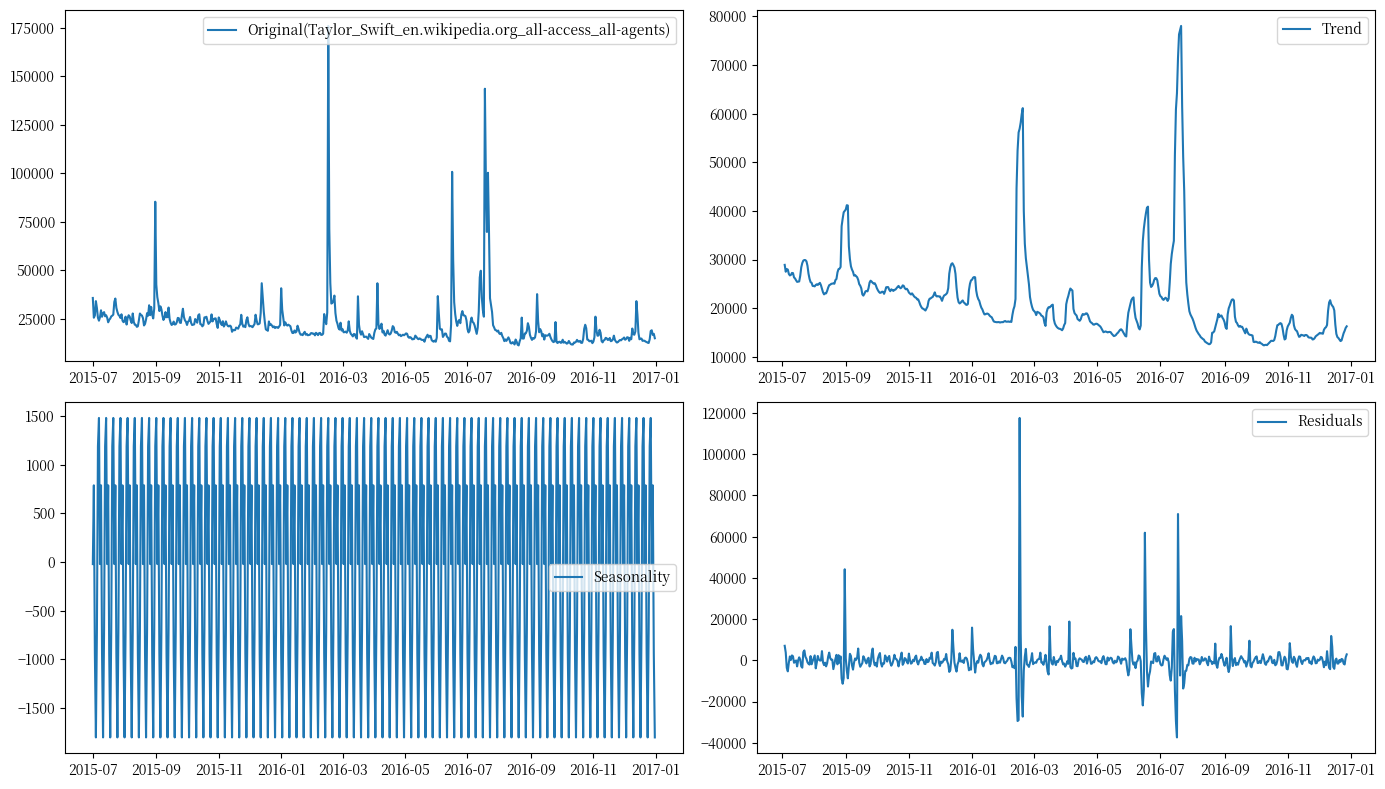
\includegraphics[width=\textwidth]{figures/Trend-decomposition.png}
  \caption{泰勒·斯威夫特趋势分解}
  \label{Trend-decomposition}
\end{figure}

(3) 假日项以及特殊因素

$h(t)$可用来反映时间序列中某时刻的特殊变动,Prophet模型根据每个假日项在不同时刻下产生的影响构建独立的模型,
并为各个假日项设置不同的前后窗口期,以及产生相应的虚拟变量\cite{JSJA2019S1097}。$h(t)$ 的表达形式如下。
\begin{align}
  h(t)&=\sum_{i=1}^{L}K_{i}1\ (t\in D_{i}), \\
  Z(t)&=[1(t\in D_{1}),...,1\ (t\in D_{L})], \\
  h(t)&=Z(t)_{k},k\sim normal(0, \gamma)
\end{align}

在现实环境中,除了周末,同样有很多节假日,而且不同的国家有着不同的假期。
在 Prophet 里面,通过维基百科里面对各个国家的节假日的描述,hdays.py 收集了各个国家的特殊节假日。
针对泰勒·斯威夫特这个词条来说,每一次专辑的发售都是一次重要的影响,发售专辑的时间可以算做一个假日。

通过加上不同影响因素,模型的准确度也会不一样。笔者通过加上不同的选项比如周期性,假日性和普通 prophet 模型加以对比,选出了效果比较好的一个模型。

\begin{figure}[htbp]
\centering
\begin{subfigure}{.5\textwidth}
  \centering
  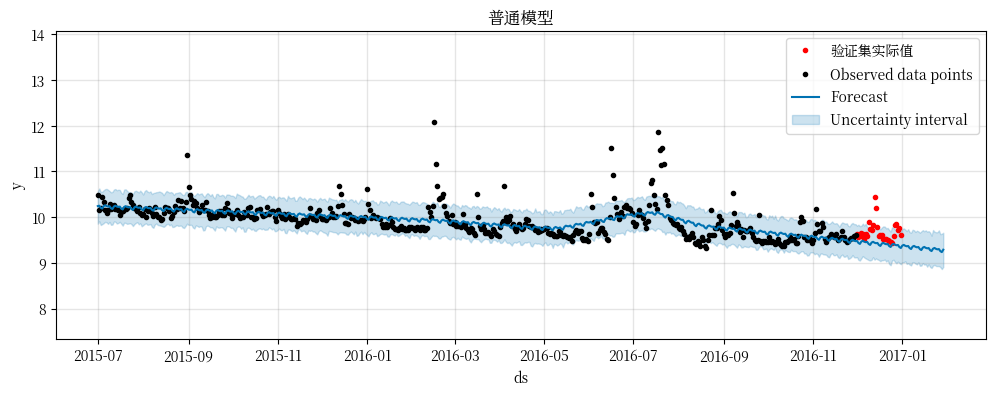
\includegraphics[width=\linewidth]{figures/prophet_normal.png}
  \caption{ProPhet 普通模型}
\end{subfigure}%
\begin{subfigure}{.5\textwidth}
  \centering
  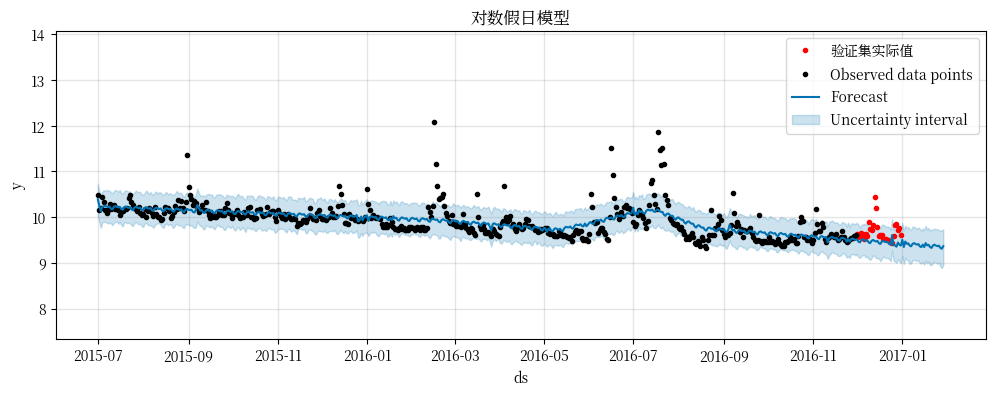
\includegraphics[width=\linewidth]{figures/prophet_holidays.png}
  \caption{Prophet 假日模型}
\end{subfigure}\\
\begin{subfigure}{\textwidth}
  \centering
  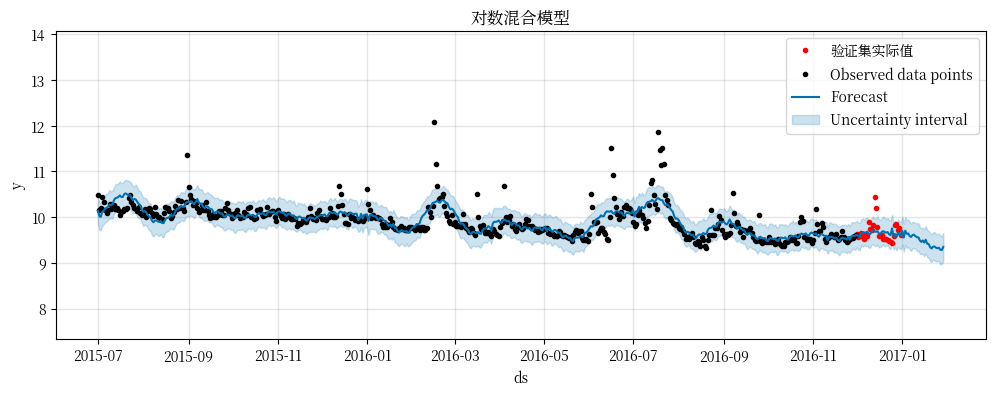
\includegraphics[width=\linewidth]{figures/prophet_mix.png}
  \caption{Prophet 混合模型}
\end{subfigure}
\caption{Prophet 几个模型的结果}
\label{compare_model}
\end{figure}

图\ref{compare_model}中,使用普通模型的 SMAPE 的分数为 0.25758,使用假日模型的 SMAPE 的分数为 0.22900,使用混合模型的 SMAPE 的分数 0.14071。SMAPE 的分数越低,代表着模型的预测性能越好。
三个图片中,小红点是验证集的实际值,小黑点显示训练集的实际值,蓝色的线代表着prophet模型的预测值,蓝色的区域是置信区间,上面是可能区间上限,下面是可能区间下限。
可以很直观的看到,仍旧存在某些没有预测到的特殊因素,需要额外的参数输入。
经过查询与泰勒·斯威夫特的新闻有很大关系。总的来说虽然蓝色的线并没有覆盖掉全部的训练集数据,但是在其他的条件下,基本有效的预测了访问量数据。
考虑了周期性和假日性的 prophet 还是没有达到最好的效果,不过勉强也可以了。

\section{两种算法的比较以及选择}

通过 SMAPE(对称平均绝对百分比误差)的比较,得到了了两个模型根据相同数据下最好的参数下的表现。但是仅仅是针对这一条数据下的表现,不具有普遍性,所以需要对每一个词条都要做拟合并预测得到每一个词条的 SAMPE 分数。
最后比较最后的平均值即可。结果如下图\ref{compare_model2}所示。

\begin{figure}[htbp]
  \centering
  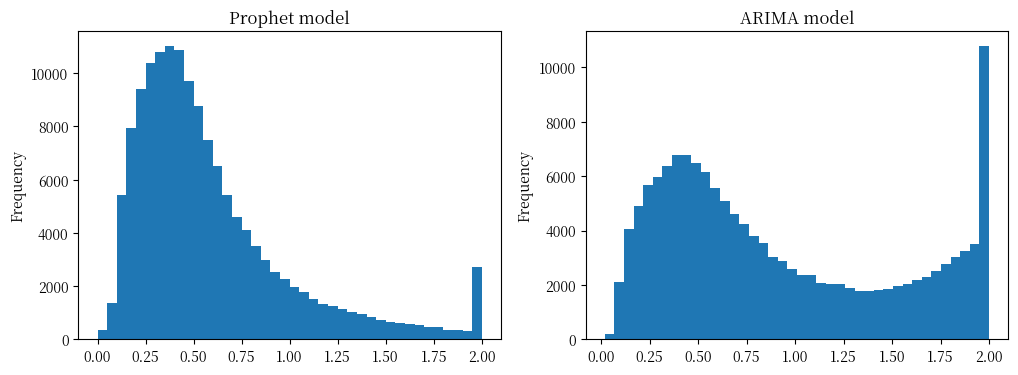
\includegraphics[width=\textwidth]{validation_compare.png}
  \caption{模型 SMAPE 分数的比较}
  \label{compare_model2}
\end{figure}

很直观的看到了两个模型的性能,prophet 的最后 SAMPE 得分为 $0.586509$,ARIMA 的最后得分为 $0.919387$。
虽然在某些个词条例如泰勒斯威夫特下表现和 prophet 的模型没有太大差异,但是没有经过一个一个对词条的参数的调整(笔者最后使用 auto\_arima 自动选择合适的词条参数),拟合结果就不尽人意,ARIMA 的预测准确度会大大下跌。
所以最后选择了考虑了周期性(季节性)、假日性、特殊因素、趋势项的 prophet 模型。

\section{本章小结}

在本章节首先介绍了数据的来源以及数据的特点,并对预测词条的时间序列做了处理。然后探讨当前常见的时间序列预测算法,决定使用 ARIMA 和近年来比较先进的 prophet 算法进行实验和探究。最后比较两个算法对所有词条的分数的平均值,结果表明prophet算法有更好的预测效果。
